%% latex_185_moulds_g.tex
%% You will need to rename this file with your information in the following format:
%% latex_185_last name_ first initial.tex
%% ------------------------------------------------------------

\documentclass[12pt,journal,compsoc]{IEEEtran}

%-----PACKAGES-------------------------------------------------

\usepackage{graphicx}
% This is an example of how a \usepackage{} command should be included. You will need to include more packages to complete this assignment.
\usepackage{verbatim}
%for hyperlink-table of contents
\usepackage{color}
\usepackage{hyperref}
\hypersetup{
    colorlinks=true, % color the links
    linkcolor=blue, % color links blue
    urlcolor=red, % color URLs red
    linktoc=all % create links for 'all' TOC items
}
\usepackage{hyperref}




%------The DOCUMENT----------------------------------------------

\begin{document}


\title{\LaTeX \hspace{1.5mm}Tutorial}
\author{Brian~Houts}
\date{}		% leaving the brackets empty omits the date
% To input the current date, you can type: \date{\today}

% The paper headers
\markboth{\LaTeX\ Tutorial}%
{Houts \MakeLowercase{\textit{et al.}}: CMPE185}
% The only time the second header will appear is for the odd numbered pages
% after the title page when using the twoside option.

\IEEEcompsoctitleabstractindextext{%
\begin{abstract}
%\boldmath
An introduction to the typesetting program \LaTeX.
\end{abstract}

\begin{IEEEkeywords}
\LaTeX, Tutorial
%CMPE185, \LaTeX\ Tutorial, IEEEtran, journal, \LaTeX, paper, template.
\end{IEEEkeywords}}

\maketitle
\tableofcontents
\newpage

%-----SECTIONS----------------------------------------------------

\section{Introduction}

\IEEEPARstart{T}{his} is tutorial for the typesetting program \LaTeX \hspace{.75mm} intended for engineering students with a little background in programming, but no previous experience in \LaTeX. \\
\indent Why learn \LaTeX? Take a second to look over this document. The tutorial itself was written using \LaTeX. Imagine for a second trying to format the equivalent in Microsoft Word. This document is formatted in IEEE standard, simply by including one simple line of code. If a different format is later desired, one simply has to change this one line. Think how painstaking that same process word be in a program like Word. \\
\indent Simply put, \LaTeX \hspace{.75mm} is to Microsoft Word as a PC is to a Mac. While a steep learning curve is there for beginners (and this tutorial is intended to help you with that), the end result is a freedom in formatting and style unmatched by other typesetting programs.
 

% Creating a subsection is similar to creating a section and is used with the command \subsection{}.

\section{Creating a .tex File}
\subsection{Preamble}
The first part of a \LaTeX\hspace{1.5mm} document is called the "preamble." After compiled the preamble does not show up on the outputted PDF since it consists of the lines before the 
\verb|\begin{document}|
environment. The preamble includes the 
\verb|\documentclass{}|
declaration and packages.
\begin{enumerate}
\item $\backslash$documentclass\{\}
\\Every \LaTeX\hspace{1.6mm}document begins with $\backslash$documentclass\{\} as it declares the type of document that you will be creating. The class is placed insode the curly brackets and Modifiers (added before the curly braces wihin square brackets [])can specify font size ([10pt], templates, and more.
\item Packages \\
Use the $\backslash$usepackage\{\} command in the preamble to include packages in your document. Packages allow for additional commands that can be used for extra formatting including math, and much, much more.
\end{enumerate}
\subsection{Environments}
The \verb|begin{}| and \verb|end{}| commands are used repeatedly in LaTeX to show where an environment begins and ends.\\
The overall environment of the file starts after the preamble and consists of:
\begin{verbatim}
\begin{document}
\end{document}
\end{verbatim}
Thus, Everything included in the file will be input between these two lines.
\subsection{Reserved Characters}
The following have a special meaning in \LaTeX
\\
\begin{tabular}{|c|c|}
\hline 
\verb|\| & indicates command \\
\hline
\verb|\\| & new line \\
\hline
\verb|#| & references argument \\
\hline
\verb|$| &  math mode\\
\hline
\verb|%| &  comment\\
\hline
\verb|{}| &  included in commands and environments\\
\hline
\verb|~| &  keep two words together n the same line\\
\hline
\verb|&| &  separates out columns in a table\\
\hline

\end{tabular}

If you want the characters to appear in the outputted PDF, use the \verb|{verbatim}| environment, or use a $\backslash$ before the character. Of course $\backslash$, itself is an exception to this rule, so one must use the command \verb|$\backslash$| .

\subsection{Title and Heading Information}

The following commands can be included in the preamble with the desired text within the curly braces \{\} to include title information in your document. In order to include this information, you must use the \verb|\maketitle| command within the document environment. \\
\begin{tabular}{|c|c|}
\hline
\verb|\title{} |& {Title} \\
\hline
\verb|\author{} |& {Author} \\
\hline
\verb|\date{} |& {date} \\
\hline
\end{tabular}




%----- Additional Features---------------------------------

\section{Additional Features}

%-------------------------
\subsection{Sections and Sub-Sections}
The \verb|\section{}| command with the desired title input between the curly braces \{\} can be used to section up your paper as in this one. This function conveniently keeps track of the number of the section for you. \\
The \verb|\subsection{}| command creates sub sections within your sections. \\
While the command \verb|\section| inserts the new section into the table of contents as well as into the navigation bars, the \verb|\section*| command only adds the section into the navigation bars.
\subsubsection{Sub-Sub-Sections}
The \verb|\subsubsection{}| command creates sub sections within subsections!

%-------------------------
\subsection{Body Text: Paragraphs and Context}
Simply writing out sentences (avoiding reserved characters) within the document environment, will result in that same text outputted into your PDF when compiled. Of Course, certain formatting commands can be useful.

\subsubsection{Stylized text formatting}
\begin{tabular}{|c|p{5cm}|}
\hline
STYLE & COMMAND \\
\hline
Bold & \verb|\textbf{}| \\
Size & \verb|\huge,  \small, ect.| \\
Underline & \verb|\underline{}| \\ 
Italicize & \verb|\textit{}| \\
\hline
\end{tabular}

\subsubsection{Justifying text}
\begin{tabular}{|c|p{5cm}|}
\hline
\verb|\centering| & centers text on page \\
\hline
\verb|\flushleft| & justifies text left  \\
\hline
\verb|\flushright| & justifies text right \\
\hline
\end{tabular} \\
Note: The above text alignment commands can also be used in an environment (\verb|\begin{flushright}}|, and if not then everything following the command will be justified accordingly.

\subsubsection{Some useful commands}
\begin{tabular}{|c|p{5cm}|}
\hline
\verb|\indent| & will indent \\
\hline
\verb|\hspace{0pt}| & adds horizantal space with the length specified in between the curly braces \{\} \\
\hline
\verb|\vspace{0pt}| & adds vertical space with the length specified in between the curly braces \{\} \\
\hline
\verb|\hline| & adds a horizontal line across page \\ 
\hline
\verb|\par| & starts new paragraph \\
\hline

\end{tabular}
%-------------------------
\subsection{Mathematical Formulas}
One of the greatest things about \LaTeX is its ability to format mathematical equations beautifully and simply.
\subsubsection{In-Line Equations}
To use mathematical equations within a line of text such as $y=x^2+5$, one can simply use math mode. That is, place the equation between two \$ symbols( i.e \verb|$y=x^2+5$|).
\subsubsection{Display Equations}
To display Mathematical equations on their own line, displayed out of the context of the paragraph describing it like the one that follows, one can use an environment.
\begin{equation}
y=x^2+5
\end{equation}
Simply start with the \verb|\begin{equation}| command and make sure to end it, after you have entered the equation, with the \verb|end{equation}| command.
\subsubsection{Symbols}
The following tables shows how one can input certain mathematical symbols in equations. Note that the commands are in math mode! Capitalizing the Greek letters simply requires capitalizing the first letter in the command.

\begin{enumerate}

\item Equality and Inequalities \\
\begin{tabular}{|c|c|}
\hline
SYMBOL & COMMAND \\
\hline
$=$ & \verb|=| \\
$\leq$ & \verb|\leq| \\
$\geq$ & \verb|\greq| \\
\hline
\end{tabular}

\item Some Greek Letters \\
\begin{tabular}{|c|c|}
\hline
SYMBOL & COMMAND \\
\hline
$\alpha$ & \verb|\alpha| \\
$\beta$ & \verb|\beta| \\
$\theta$ & \verb|\theta| \\
$\epsilon$ & \verb|\epsilon| \\
$\mu$ & \verb|\mu| \\
$\pi$ & \verb|\pi| \\
$\Delta$ & \verb|\Delta| \\
$\omega$ & \verb|$\omega$| \\
$\Sigma$ & \verb|$\Sigma$| \\
\hline
\end{tabular}
\end{enumerate}


\subsubsection{Fractions}
Look how beautifully \LaTeX \hspace{.5mm} can display fractions!
\begin{equation}
\frac{(50x^3+y)(\frac{1}{2}+32y^{10})}{y-10}
\end{equation}
To format a fraction, first enter math mode (whether in-line or in the equation environment) and use the \verb|\frac{}{}| command. The numerator goes in the first pair of curly braces \{\}, and the denominator goes in the second. Voila!

\subsubsection{Superscripts and Subscripts}
To use superscripts/subscripts you must first be in math mode. \\
To write a superscript (such as $10^{th}$) use a "carrot" followed by curly braces \verb|^{}|. \\
To write a superscript (such as $F_{i}$) use an "underscore" followed by curly braces \verb|_{}|. \\

%-------------------------------------------------------------------------------------------------
\subsection{Label, Cite, and Ref Commands}
You will need to be able to define and explain how to use the following commands:
\begin{verbatim} \label{fig_slug} \end{verbatim} as it appears in the figure environment\\
\begin{verbatim} \cite{IEEEhowto:kopka} \end{verbatim} appears like: \cite{IEEEhowto:kopka}\\
\begin{verbatim} \ref{fig_slug} \end{verbatim} appears like: \ref{fig_slug}\\

% IMPORTANT NOTE: In order to assign the correct reference number to each label, you may have to compile your code twice. 

%-------------------------------------------------------------------------------------------------
\subsection{Tables}
This section shows how to create tables in \LaTeX
\subsubsection{Table vs Tabular}
The \verb|\begin{tabular}| environment is the simplest way to create a table. So then what does the \verb|\begin{table}| environment do? It creates what is called a float table environment. With this, one can position the table very easily on the page as desired. Thus, much of the time "tabular" environments are placed inside "table" environments."
\subsubsection{Tabular}
The "tabular" environment is the simplest way to create a table. The form is as follows:
\begin{verbatim}
\begin{tabular}{ |c|c|c| } 
 \hline
 1 & 2 & 3 \\ 
 4 & 5 & 6 \\ 
 7 & 8 & 9 \\ 
 \hline
\end{tabular}
\end{verbatim}
The above code, creates the following table:
\begin{tabular}{ |c|c|c| } 
 \hline
 1 & 2 & 3 \\ 
 4 & 5 & 6 \\ 
 7 & 8 & 9 \\ 
 \hline
\end{tabular} \\
So the first line creates 3 columns, denoted by the 4 "bars" |, with each item centered in the columns, prompted by the 'Cs' between the "bars." The \verb|\hline| command creates a horizontal line, and we see the ones included in the code correspond to the top and bottom of the tale to be lined. each row is separated by the new line command (\verb|\\|), and \verb|&| symbols within each row separate out the columns.
\par
So what other options do we have besides the "c" that centers the text inside the table?
\begin{tabular}{ |c|p{5.5cm}| } 
 \hline
 c & centers text \\ 
 \hline
 l & left justified  \\ 
 \hline
 r & righ justified  \\ 
 \hline
 p\{width\} & replace "width" with the desired width of a paragraph  \\ 
 \hline
\end{tabular} \\


\subsubsection{Table}
The "float table" environment can be used to easily position tables on the page, as well as add titles and footnotes. The following example positions  table "here" (where the code is in the document) and in the center horizontally.
\begin{verbatim}
\begin{table}[h!]
\caption{An Example of a Table}
\label{table}
\centering
 \begin{tabular}{||c c c ||} 
 \hline
 1 & 2 & 3 \\ 
 4 & 5 & 6 \\ 
 7 & 8 & 9 \\ 
 \hline [1ex] 
 \hline
 \end{tabular}
\end{verbatim} \\
The above code creates the floating table:

\begin{table}[h!]
\centering
\caption{An Example of a Table}
\label{}
 \begin{tabular}{||c c c ||} 
 \hline
 c1 & c2 & c3 \\ [0.5ex] 
 \hline\hline
 tables & are & pretty \\ 
 fun & to & make  \\ 
 \hline 
 \end{tabular} \\
\end{table}

\subsubsection{Placement for both Tables and Figures} 


\centering
 \begin{tabular}{|||c || p{5.5cm} |||} 
 \hline
  h & place table here   \\ 
 \hline
 t & place at the top of the page   \\ 
 \hline
 b & place at the bottom of the page   \\ 
 \hline
 p & place table on a page just for tables    \\ 
 \hline
 ! &   ignore \LaTeX rules \\ 
 \hline
 H & place precisely here   \\ 
 \hline
 \end{tabular} \\
\flushleft



%--------FIGURES-----------------
\subsection{Figures}
One can add a figure to a document using the \verb|\begin{figure}| environment. Much like the "floating table" environment, one can use the \verb|\caption{}| and \verb|\label{}|. \\
The following code can be used to place a figure in a \LaTeX document. The \verb|\includegraphics[scale=•]{•}| command imports a picture into the document, as long as the image is placed inside of the directory corresponding to your \LaTeX\hspace{.5mm} file.

\begin{figure}[h!] 
\centering
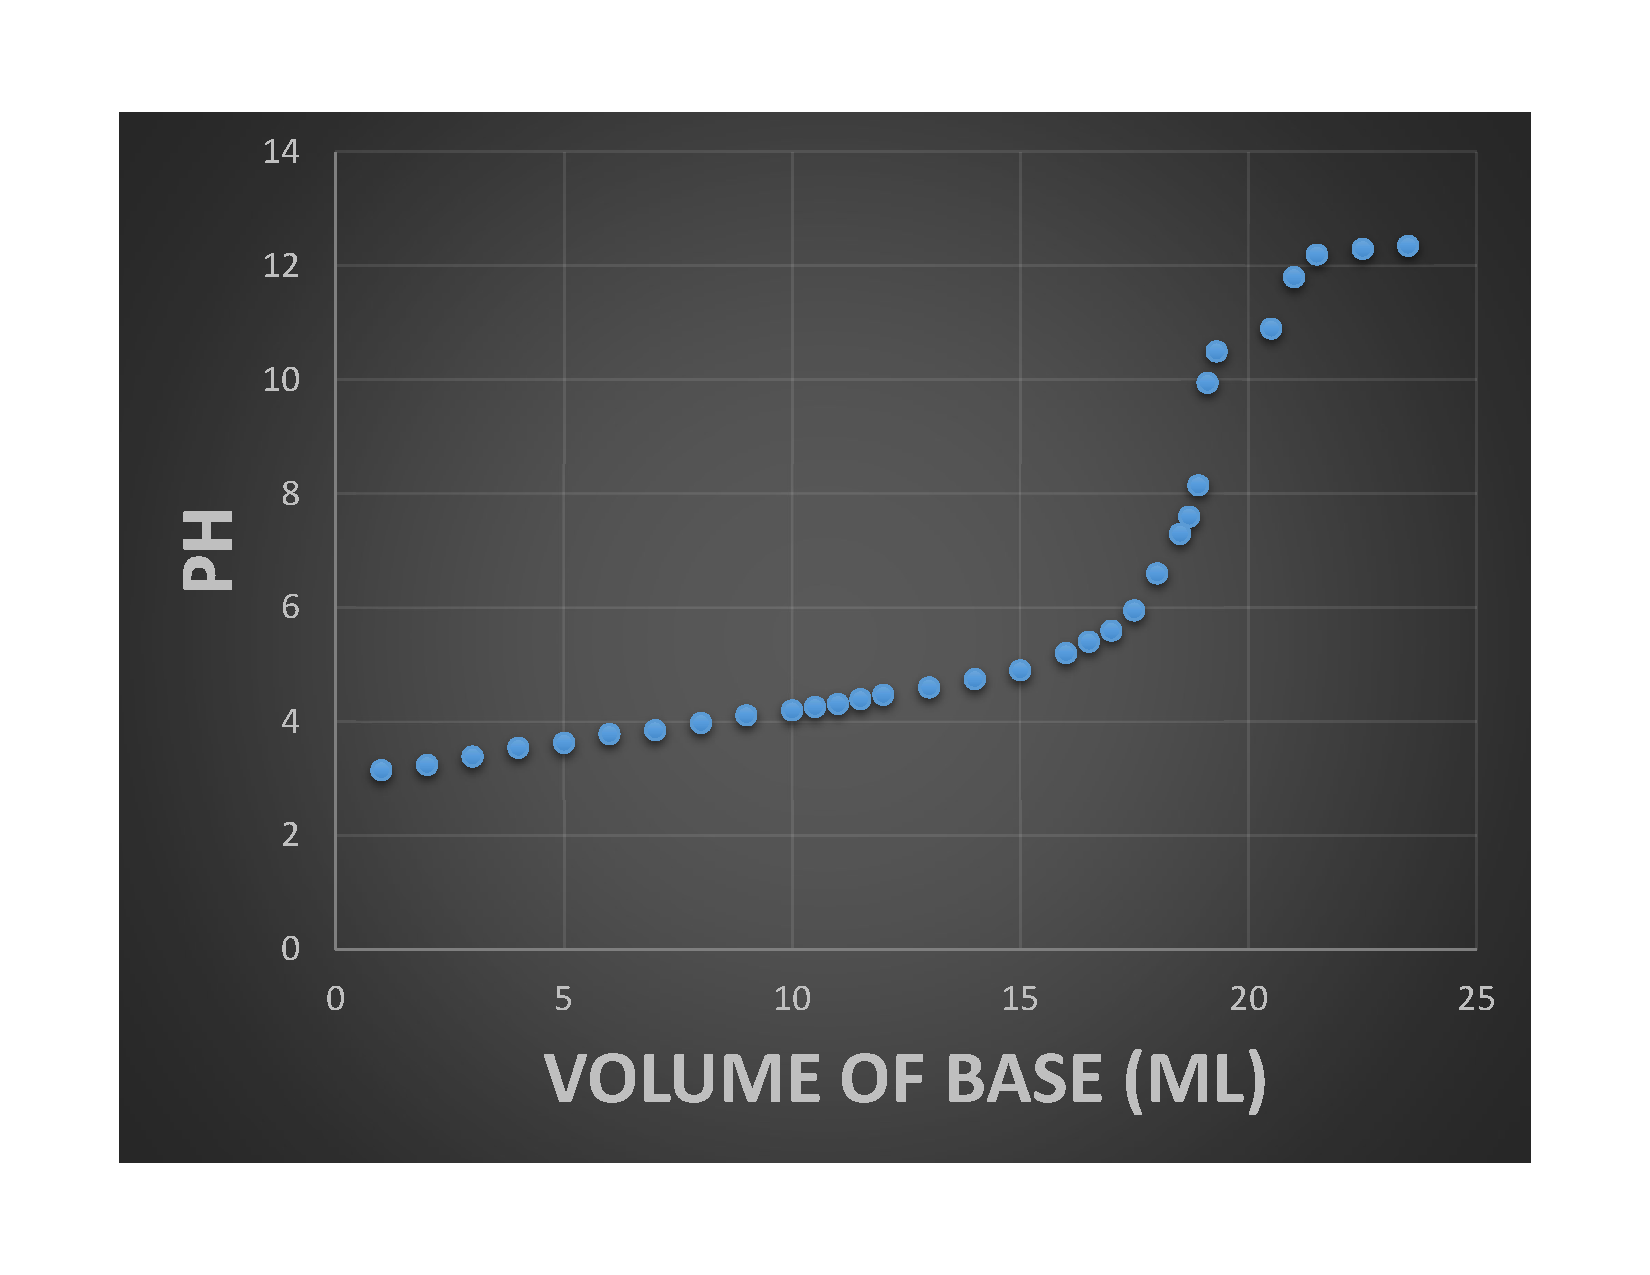
\includegraphics[width=4in]{t_plt.pdf}
\caption{This Titration Plot shows the pH of NaOH as one increases the concentration of the strong base NaOH in a weak acid. One can use the equivalence point (middle of the sharp rise) and its corresponding y-value to find NaOH's pH.}
\end{figure}
\begin{small}

\begin{verbatim}
\begin{figure}[h!] 
\centering
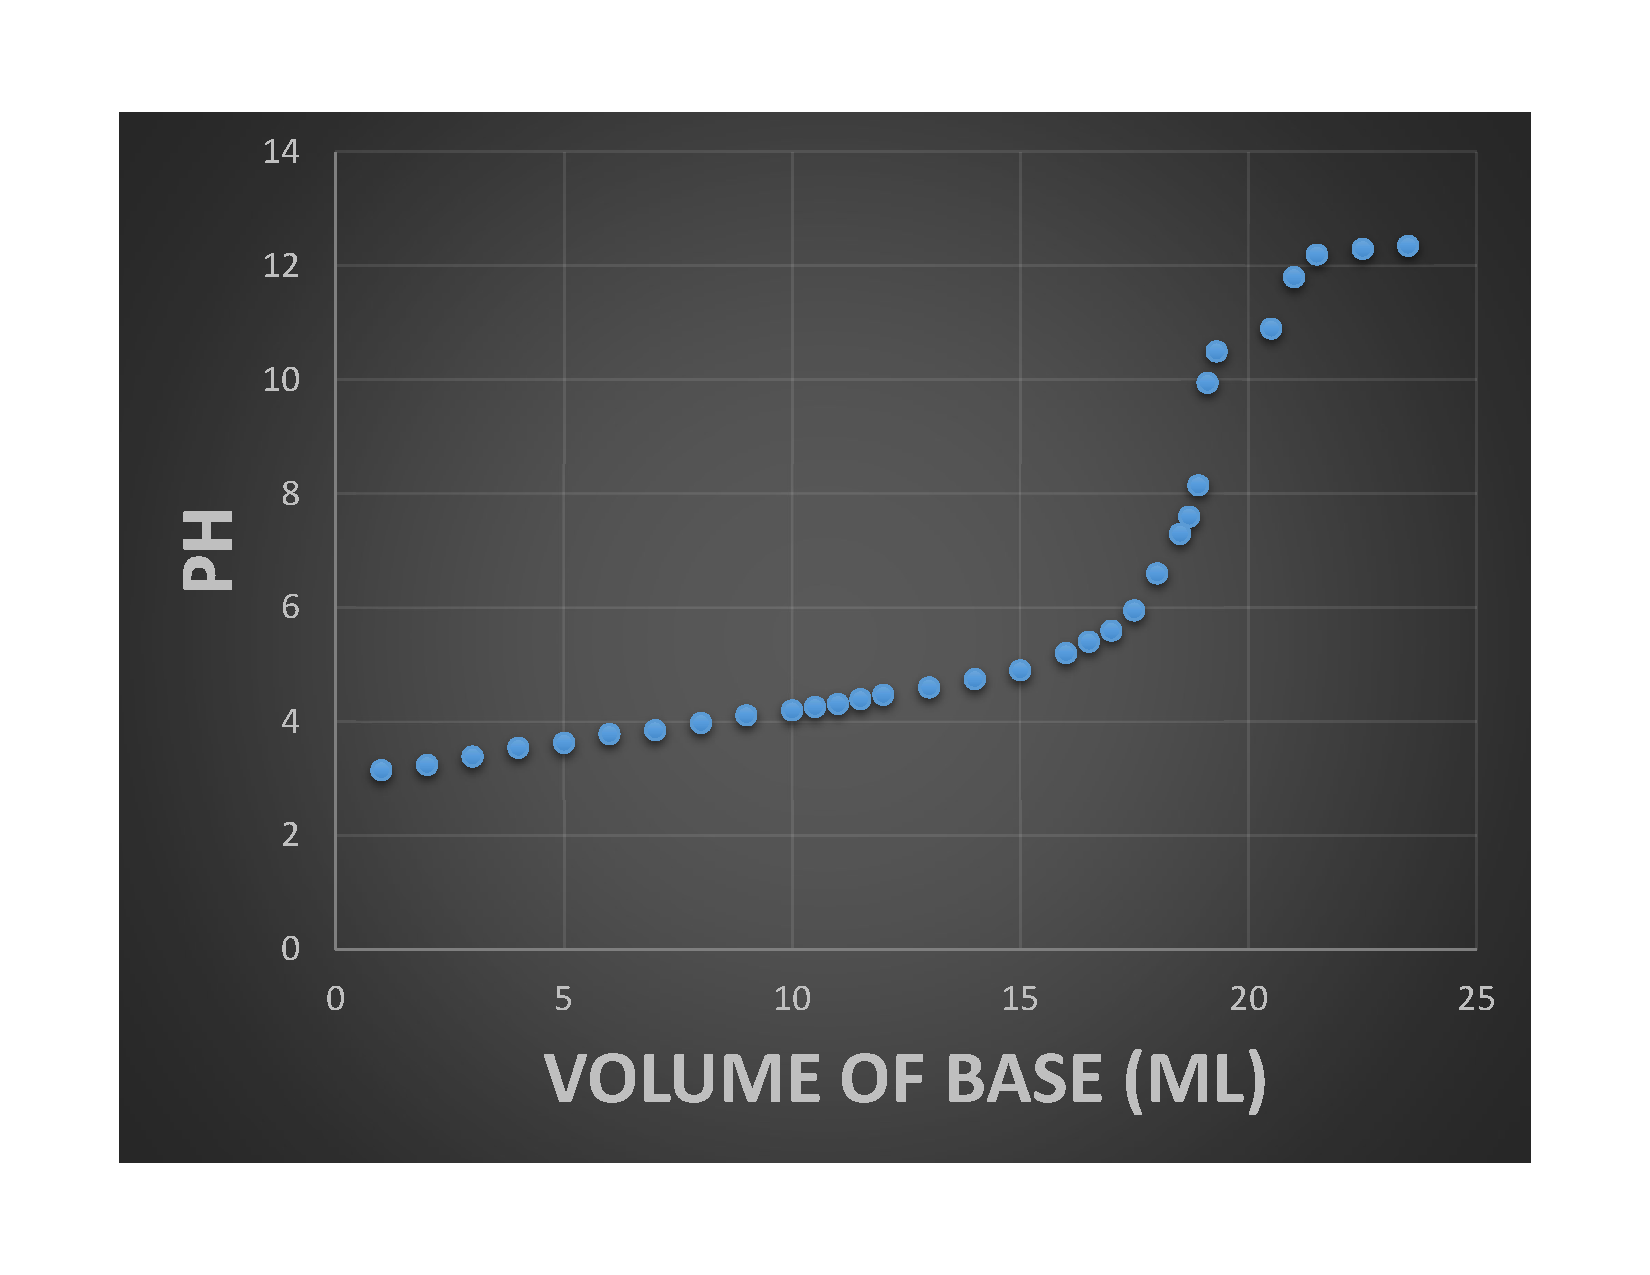
\includegraphics[width=4in]{t_plt.pdf}
\caption{This Titration Plot shows 
the pH of NaOH as one increases the 
concentration of the strong base NaOH 
in a weak acid. One can use the equivalence
 point (middle of the sharp rise) and its
 corresponding y-value to find NaOH's pH.}
\end{figure}
\end{verbatim} 
\end{small}

The above code looks for \verb|"t_plt.pdf"| within your directory and places a 4" wide figure in your file:




%----- ACKNOWLEDGEMENT SECTION -------------------------------------------------------------------
\section{How To: Acknowledgments}
An acknowledgment section is really up to the author's discretion.In \LaTeX\hspace{.5mm} I would advise having it as its own section using the \verb|\section{}| command. After that you can choose to acknowledge how you choose whether it be in list or paragraph form.

%----- BIBLIOGRAPHY--------------------------------------------
\section{How To: References}
One of the greatest functions of \LaTeX comes into play when adding a bibliography to your document. This is because if you decide you need to change the style of bibliography you can simply change one command instead of having to go through and changing each separate one! 

Depending on the document class of your document you may need to include the
a bibliography package in your preamble. In many cases, such as the IEEE class that I used in this document, it is built in. In this tutorial I will explain how to create bibliographies using the \verb|\usepackage{biblatex}| package (one of many).

\subsection{biblatex}
\begin{enumerate}
\item use these two commands in your preamble:
\begin{enumerate}
\item \verb|\usepackage{biblatex}|
\item \verb|\addbibresource{ex.bib}|
\end{enumerate} 
\item include data file (ex.bib) with bibliographies in directory containing your .tex file

\subsubsection{.bib File}
The .bib file is in the following format:
\begin{figure}[h] 
\centering
\includegraphics[width=4in]{ex_bib.pdf}
\caption{From ShareLaTeX.com: \cite{bib_ex} }
\end{figure}


\item use the \verb|\cite{example}| and \ref{example}|command within your document to include your "example" bibliography with a reference number in your document from your .bib file
\item at the  end of your document include the \verb|\printbibliography| command
\end{enumerate}
%----- CONCLUSION-----------------------------------------------
\section{Conclusion}
Well, I hoped you found this tutorial useful! I acknowledge that the possibilities in \LaTeX\hspace{.5mm} are endless, which makes it so great, and as a result this tutorial inevitably is missing information you will deem important going forward. Fortunately there is also endless documentation on the subject and a simple Google search should yield answers. Furthermore, much work will be done for you if you can find and include the right packages and class files. Go forth and create beautiful documents!



%----- ACKNOWLEDGEMENT SECTION -------------------------------------------------------------------
\section{Acknowledgements}

The author would like to thank...
\vspace{.5cm}
\begin{enumerate}
\item Gerald Moulds, for providing a template for which to work off of!
\item TIMMURPHY.ORG, in teaching me how to create a linkable Table of Content
\item SHARE\LaTeX.com, for refreshing my memory on pretty much everything in this tutorial!
\item Google! What would we do without it?

\end{enumerate}









%----- BIBLIOGRAPHY ----------------------------------------
% You will need to explain how to include the bibliography section as follows. Explain the environment and how to add new items.
% Including how \ref, \cite and \label should be included here.

% Reminder: you will need to explain how to include the Bibliography Section and then include your own Bibliography at the end of your own tutorial.
\begin{thebibliography}{1}

\bibitem{IEEEhowto:kopka}
H.~Kopka and P.~W. Daly, \emph{A Guide to {\LaTeX}}, 3rd~ed.\hskip 1em plus
  0.5em minus 0.4em\relax Harlow, England: Addison-Wesley, 1999.
 
 \bibitem{bib_ex}
Anonymous (2016), \emph{Bibliography management in LaTeX}, Available: \url{https://www.sharelatex.com/learn/Bibliography_management_in_LaTeX}

\bibitem{bib_ex}
Anonymous (2016), \emph{LaTeX table of contents with clickable links}, Available: \url{http://timmurphy.org/2014/03/11/latex-table-of-contents-with-clickable-links/}

\bibitem{bib_ex}
Anonymous (2016), \emph{Special Symbols in LaTeX}, Available: \url{https://www.noao.edu/noaoprop/help/symbols/}



\end{thebibliography}



\end{document}